% Provenance (never printed): see sources/outline_sources.md (Year 2: humidity variables;
% Clausius--Clapeyron applied; dry and moist adiabats; thermodynamic diagrams; convective
% instability; cloud microphysics). Definitions after the NWS glossary; skew-T lines, CAPE classes
% and the lifted index after the NWS Houston/Galveston training page; saturation data from the
% NIST WebBook (IAPWS-95) and IAPWS R14-08; the empirical formula as used by Su and others
% (2026); kappa-Koehler theory after Petters and Kreidenweis (2007); CCN numbers after Andreae
% (2009); the processes of microphysics after Morrison and others (2020). The sounding is the
% real 12 UTC sounding of Norman, Oklahoma, 16 April 2026 (IGRA2); every curve and number from
% figdata/bachelor-2/thermo.py; exercise and problem values in the Book 4 scratch calculator
% calc/ch21.py.
\chapter{वायुमंडलीय ऊष्मागतिकी}\label{ch:b2:atmospheric-thermodynamics}

16 अप्रैल 2026 को, 12 UTC पर, नॉर्मन, ओक्लाहोमा के मौसम केंद्र से एक गुब्बारा उठा, जैसे
हर दिन उसी समय आठ सौ से अधिक केंद्रों से गुब्बारे उठते हैं। उसके साथ गए उपकरण ने
रेडियो द्वारा एक ऊर्ध्वाधर परिच्छेदिका वापस भेजी जिसे पूर्वानुमानकर्ता एक नज़र में पढ़ लेता है: भूमि के पास वायु
लगभग संतृप्त, छह सौ मीटर ऊपर एक पतला गर्म ढक्कन, और उसके ऊपर दस किलोमीटर तक
तेज़ी से गिरता तापमान। ढक्कन के पार उठाए जाने पर सतह की वायु क्षोभमंडल के अधिकांश भाग में
अपने परिवेश से गर्म होती, और उसके पास उठने पर ख़र्च करने के लिए प्रति किलोग्राम कोई दो हज़ार जूल
होते। यह अध्याय उस ऊर्जा को एक साउंडिंग से पढ़ना सीखता है: वायु कितना
जल रखती है, उठता वायु-पिंड संघनन से पहले और बाद में कैसे ठंडा होता है, मौसमविज्ञानियों के आरेख
क्षेत्रफलों को ऊर्जाओं में कैसे बदलते हैं, और मेघ-बूँदें बनती ही कैसे हैं।
% ledger: data:b4-sounding, nws4:upperair, nws4:cape

\begin{recall}
\textbf{भौतिकी की पुस्तकों से}: संतृप्त \omterm{def:b2:atmospheric-thermodynamics:moist-air}{वाष्प दाब}, सापेक्ष आर्द्रता, ओसांक,
गुप्त ऊष्मा, क्लॉसियस--क्लेपेरॉन संबंध और उसका समाकलित रूप; नाभिकन और
अतिशीतलन; प्रथम नियम, रुद्धोष्म परिवर्तन और आदर्श गैस की ऊष्मा धारिताएँ।
\textbf{रसायन विज्ञान की पुस्तकों से}: आंशिक दाब, राउल्ट का नियम, पृष्ठ तनाव और केल्विन
समीकरण। \textbf{स्कूल की पुस्तकों से}: \omterm{def:b2:atmospheric-thermodynamics:lcl}{संघनन तल} और उसका प्रति अंश
\qty{125}{m} का नियम, स्थिर और अस्थिर वायु, \omterm{def:b2:atmospheric-thermodynamics:microphysics}{संघनन केंद्रक}, उष्ण-वर्षा और
हिम-क्रिस्टल प्रक्रम। \textbf{पुस्तक 3 (स्नातक वर्ष 1) से}: मानक वायुमंडल, परिवेशी
और शुष्क रुद्धोष्म तापह्रास दरें ($\Gamma_d = \qty{9.8}{K/km}$), वायु-पिंड, विभव
तापमान, स्थैतिक स्थिरता, तापमान-व्युत्क्रमण और हिप्सोमेट्रिक समीकरण।
\end{recall}

पूरे अध्याय में: $R_d = R/M_d = \qty{287.0}{J.kg^{-1}.K^{-1}}$, शुष्क वायु के लिए, जिसका मोलर द्रव्यमान \qty{28.97}{g/mol} है;
$R_v = R/M_w = \qty{461.5}{J.kg^{-1}.K^{-1}}$, जल-वाष्प के लिए, जिसका मोलर द्रव्यमान \qty{18.0153}{g/mol} है;
$\varepsilon = M_w/M_d = 0.622$; $c_p = \tfrac72 R_d =
\qty{1004.5}{J.kg^{-1}.K^{-1}}$ (पुस्तक 3, ऊष्मा धारिताओं के अनुपात 1.4 के साथ);
$g = \qty{9.81}{m.s^{-2}}$; और त्रिक बिंदु पर वाष्पन की गुप्त ऊष्मा,
$L = \qty{2.501e6}{J/kg}$।
% ledger: const:R, earth:Mmol, nist4:water-mw, nasa:grc-gamma, const:gn, nist4:water-sat

\section{आर्द्र वायु}\label{sec:b2:atmospheric-thermodynamics:moist-air}

वायु शुष्क वायु और जल-वाष्प का मिश्रण है, दोनों आदर्श गैसों के निकट। भौतिकी की पुस्तकें
उसके जल को सापेक्ष आर्द्रता और ओसांक से मापती हैं; उठते वायु-पिंड को ऐसे मापों की आवश्यकता है
जो उसके फैलने पर न बदलें।

\begin{definition}[वाष्प दाब; मिश्रण-अनुपात; विशिष्ट आर्द्रता]\label{def:b2:atmospheric-thermodynamics:moist-air}
आर्द्र वायु का \emph{वाष्प दाब}\index{वाष्प दाब} $e$ उसकी जल-वाष्प का आंशिक दाब
है। उसका \emph{मिश्रण-अनुपात}\index{मिश्रण-अनुपात} $r = m_v/m_d$ है, यानी उसी आयतन में शुष्क वायु के प्रति इकाई द्रव्यमान
जल-वाष्प का द्रव्यमान, और उसकी \emph{विशिष्ट
आर्द्रता}\index{विशिष्ट आर्द्रता} $q = m_v/(m_d + m_v)$ है, यानी आर्द्र वायु के प्रति इकाई द्रव्यमान
वाष्प का द्रव्यमान। दोनों सामान्यतः ग्राम प्रति किलोग्राम में दिए जाते हैं।
\end{definition}
% ledger: nws4:humidity

\begin{proposition}[आर्द्रता के चर]\label{prop:b2:atmospheric-thermodynamics:humidity}
कुल दाब $p$ और \omterm{def:b2:atmospheric-thermodynamics:moist-air}{वाष्प दाब} $e$ वाली आर्द्र वायु में,
\[
  r = \frac{\varepsilon e}{p - e}, \qquad q = \frac{r}{1 + r} = \frac{\varepsilon e}{p - (1 -
  \varepsilon)e} .
\]
संतृप्ति पर $e = e_s(T)$ और $r = r_s(T, p)$, संतृप्ति \omterm{def:b2:atmospheric-thermodynamics:moist-air}{मिश्रण-अनुपात}। जब कोई वायु-पिंड जल पाए या खोए बिना
फैलता या संपीडित होता है, तब न $r$ बदलता है न $q$।
\end{proposition}

\begin{proof}
उसी आयतन $V$ में तापमान $T$ पर, हर गैस अपने आंशिक दाब के साथ अपने आदर्श-गैस नियम का पालन करती है:
$m_v = eV/(R_vT)$ और $m_d = (p - e)V/(R_dT)$, इसलिए $r = (R_d/R_v)\,e/(p - e)$,
और $R_d/R_v = M_w/M_d = \varepsilon$। $m_v$ को $m_d + m_v$ से भाग देने पर $q = r/(1 + r)$ मिलता है।
प्रसार $V$, $p$ और $e$ को बदलता है पर दोनों द्रव्यमानों को नहीं।
\end{proof}

\begin{definition}[आभासी तापमान]\label{def:b2:atmospheric-thermodynamics:virtual}
आर्द्र वायु का \emph{आभासी तापमान}\index{आभासी तापमान} $T_v$ वह तापमान है
जो शुष्क वायु को, उसी दाब पर, उसी घनत्व के लिए चाहिए:
\[
  T_v = T\,\frac{1 + r/\varepsilon}{1 + r} \approx T\,(1 + 0.61\,r) .
\]
\end{definition}
% ledger: nws4:virtual-theta-e

यह तापमान जो कहता है वही करता है, इसकी उपपत्ति एक पंक्ति है: आर्द्र वायु का घनत्व
$(m_d + m_v)/V = \bigl(p - e\bigr)/(R_dT) + e/(R_vT)$ है, जो $e = pr/(\varepsilon + r)$ के साथ
$p/(R_dT_v)$ के बराबर है। जल-वाष्प शुष्क वायु से हल्की है, इसलिए उसी तापमान और दाब पर आर्द्र वायु शुष्क
वायु से कम घनी होती है, मानो वह थोड़ी गर्म हो।

\begin{example}[नॉर्मन की वायु]\label{ex:b2:atmospheric-thermodynamics:norman}
भूमि पर साउंडिंग $p = \qty{971.1}{hPa}$, $T = \qty{19.0}{\celsius}$ और
\qty{18.5}{\celsius} का ओसांक देती है। \omterm{def:b2:atmospheric-thermodynamics:moist-air}{वाष्प दाब} ओसांक पर का संतृप्त \omterm{def:b2:atmospheric-thermodynamics:moist-air}{वाष्प दाब} है,
$e = e_s(\qty{18.5}{\celsius}) = \qty{21.5}{hPa}$ (नीचे \cref{prop:b2:atmospheric-thermodynamics:es})।
तब $r = 0.622 \times 21.5/(971.1 - 21.5) = \qty{14.1}{g/kg}$, $q = \qty{13.9}{g/kg}$,
और $T_v - T = 0.61 \times 0.0141 \times \qty{292.15}{K} = \qty{2.5}{K}$: यह वायु उतनी ही हल्की है जितनी
ढाई अंश अधिक गर्म शुष्क वायु।
\end{example}
% ledger: data:b4-sounding

\section{संतृप्त वाष्प दाब}\label{sec:b2:atmospheric-thermodynamics:saturation}

शुद्ध जल की एक समतल सतह के ऊपर साम्य पर \omterm{def:b2:atmospheric-thermodynamics:moist-air}{वाष्प दाब} केवल तापमान पर निर्भर करता है।
भौतिकी की पुस्तकें उसका नियम, क्लॉसियस--क्लेपेरॉन संबंध, व्युत्पन्न करती हैं और उसे
स्थिर गुप्त ऊष्मा के साथ समाकलित करती हैं; जल-वाष्प के लिए $M L/R = L/R_v$।

\begin{proposition}[संतृप्त वाष्प दाब]\label{prop:b2:atmospheric-thermodynamics:es}
गुप्त ऊष्मा $L$ को स्थिर रखने पर, जल के ऊपर संतृप्त \omterm{def:b2:atmospheric-thermodynamics:moist-air}{वाष्प दाब} है
\[
  e_s(T) = e_t \exp\!\Bigl[\frac{L}{R_v}\Bigl(\frac{1}{T_t} - \frac{1}{T}\Bigr)\Bigr],
  \qquad e_t = \qty{6.117}{hPa}, \quad T_t = \qty{273.16}{K}, \quad \frac{L}{R_v} =
  \qty{5419}{K},
\]
जहाँ $(T_t, e_t)$ जल का त्रिक बिंदु है।
\end{proposition}
% ledger: iapws4:sublimation, nist4:water-sat

\begin{corollary}[प्रति केल्विन सात प्रतिशत]\label{cor:b2:atmospheric-thermodynamics:seven}
संतृप्त \omterm{def:b2:atmospheric-thermodynamics:moist-air}{वाष्प दाब} की वृद्धि की सापेक्ष दर
$\mathrm{d}\ln e_s/\mathrm{d}T = L/(R_v T^2)$ है:
\qty{7.3}{\percent} प्रति केल्विन, \qty{0}{\celsius} पर;
\qty{6.3}{\percent}, \qty{20}{\celsius} पर; \qty{5.9}{\percent}, \qty{30}{\celsius} पर।
\end{corollary}

स्थिर गुप्त ऊष्मा सूत्र का एकमात्र दोष है: गुप्त ऊष्मा त्रिक बिंदु पर के
\qty{2500.9}{kJ/kg} से गिरकर \qty{2453.5}{kJ/kg} हो जाती है, \qty{20}{\celsius} पर, इसलिए तापमान बढ़ने के साथ
सूत्र मापे गए मानों से आगे निकल जाता है: \qty{1.2}{\percent}, \qty{20}{\celsius} पर, और
\qty{2.5}{\percent}, \qty{30}{\celsius} पर (नीचे का चित्र)। मापों पर बिठाया गया एक आनुभविक
सूत्र, $e_s = \qty{6.112}{hPa} \times \exp[17.67\,t/(t + 243.5)]$, जहाँ
$t$ डिग्री सेल्सियस में है, हज़ार में कुछ भागों के भीतर रहता है; आँकड़ा-उत्पाद उसका उपयोग करते हैं, पर
प्रस्ताव वह है जिसका अवकलन किया और जिसे समझा जा सकता है, और यह अध्याय उसी को रखता है।
% ledger: nist4:water-sat, su26:svp

\qty{0}{\celsius} से नीचे मेघों में जल द्रव, अतिशीतित, रह सकता है, और दो संतृप्त
\omterm{def:b2:atmospheric-thermodynamics:moist-air}{वाष्प दाब} होते हैं: द्रव जल के ऊपर और हिम के ऊपर। दूसरा कम है, क्योंकि ऊर्ध्वपातन की गुप्त
ऊष्मा वाष्पन की गुप्त ऊष्मा से संगलन की गुप्त ऊष्मा जितनी अधिक है। अतिशीतित बूँदों के सापेक्ष संतृप्त वायु
हिम के सापेक्ष अतिसंतृप्त होती है: \qty{10}{\percent}, \qty{-10}{\celsius} पर, और
\qty{22}{\percent}, \qty{-20}{\celsius} पर: अंतिम खंड इस अंतर पर
लौटता है।
% ledger: iapws4:sublimation, su26:svp

\begin{omfigure}
\centering
% figdata/bachelor-2/thermo.py parts es, nist
\begin{tikzpicture}
\begin{groupplot}[group style={group size=2 by 1, horizontal sep=1.9cm},
  width=0.44\linewidth, height=5.4cm, tick label style={font=\scriptsize},
  label style={font=\small}]
\nextgroupplot[xmin=-40, xmax=40, ymin=0, ymax=80, xlabel={तापमान (\unit{\celsius})},
  ylabel={संतृप्त वाष्प दाब (\unit{hPa})}, legend pos=north west,
  legend style={font=\scriptsize, draw=none, fill=none}, legend cell align=left]
\addplot[ocBlue, thick] table[x=T_C, y=cc] {figdata/out/bachelor-2-thermo-es.dat};
\addlegendentry{प्रस्ताव}
\addplot[black, densely dashed] table[x=T_C, y=emp] {figdata/out/bachelor-2-thermo-es.dat};
\addlegendentry{आनुभविक सूत्र}
\addplot[only marks, mark=*, mark size=1.4pt, ocRed] table[x=T_C, y=es_hPa]
  {figdata/out/bachelor-2-thermo-nist.dat};
\addlegendentry{मापित (IAPWS-95)}
\nextgroupplot[xmin=-40, xmax=0, ymin=1, ymax=1.5, xlabel={तापमान (\unit{\celsius})},
  ylabel={$e_s(\text{जल})/e_s(\text{हिम})$}]
\addplot[omMeth, thick, unbounded coords=discard] table[x=T_C, y=wi]
  {figdata/out/bachelor-2-thermo-es.dat};
\draw[black!40, densely dotted] (axis cs:-10,1) -- (axis cs:-10,1.1035) -- (axis cs:-40,1.1035);
\node[font=\scriptsize, anchor=south west] at (axis cs:-10,1.1035) {1.10};
\draw[black!40, densely dotted] (axis cs:-20,1) -- (axis cs:-20,1.218) -- (axis cs:-40,1.218);
\node[font=\scriptsize, anchor=south west] at (axis cs:-20,1.218) {1.22};
\end{groupplot}
\end{tikzpicture}
\par\smallskip{\small बायाँ: जल के ऊपर संतृप्त \omterm{def:b2:atmospheric-thermodynamics:moist-air}{वाष्प दाब},
\cref{prop:b2:atmospheric-thermodynamics:es} से, आनुभविक सूत्र से और जैसा मापा गया। दायाँ:
अतिशीतित जल (आनुभविक सूत्र) और हिम (IAPWS ऊर्ध्वपातन समीकरण) के ऊपर संतृप्त वाष्प दाबों का
अनुपात।}
\end{omfigure}
% ledger: nist4:water-sat, iapws4:sublimation, su26:svp

\section{उठती आर्द्र वायु}\label{sec:b2:atmospheric-thermodynamics:ascent}

ऊष्मा का आदान-प्रदान किए बिना उठता वायु-पिंड शुष्क रुद्धोष्म तापह्रास दर से ठंडा होता है, अपना
विभव तापमान बनाए रखता है, और, यदि संघनित न हो, अपना \omterm{def:b2:atmospheric-thermodynamics:moist-air}{मिश्रण-अनुपात} बनाए रखता है। उसका \omterm{def:b2:atmospheric-thermodynamics:moist-air}{वाष्प दाब}
$e = pr/(\varepsilon + r)$ दाब के साथ गिरता है, पर उसका संतृप्त \omterm{def:b2:atmospheric-thermodynamics:moist-air}{वाष्प दाब} अपने तापमान के साथ
और तेज़ी से गिरता है। दोनों एक ऐसे तल पर मिलते हैं जिसे स्कूल की पुस्तकों ने एक नियम से पाया था।

\begin{definition}[उत्थापन संघनन तल]\label{def:b2:atmospheric-thermodynamics:lcl}
किसी वायु-पिंड का \emph{उत्थापन संघनन तल}\index{उत्थापन संघनन तल} (LCL) वह
तल है जिस पर शुष्क-रुद्धोष्म रूप से उठाए जाने पर वह संतृप्त हो जाता है। यही स्कूल की पुस्तकों का
\emph{संघनन तल}\index{संघनन तल} है, उठाव से बनने वाले मेघों के
सपाट आधारों की ऊँचाई।
\end{definition}
% ledger: nws4:lcl

\begin{proposition}[उत्थापन संघनन तल की ऊँचाई]\label{prop:b2:atmospheric-thermodynamics:lcl}
तापमान $T$ और ओसांक $T_d$ वाला वायु-पिंड लगभग इतनी ऊँचाई पर संतृप्ति तक पहुँचता है:
\[
  z_{\text{LCL}} \approx \frac{T - T_d}{\Gamma_d - \Gamma_{\text{ओस}}}, \qquad
  \Gamma_{\text{ओस}} = \frac{g R_v T_d^2}{L R_d T} \approx \qty{1.8}{K/km},
\]
अपने आरंभिक तल से ऊपर: ओसांक-अवनमन के प्रति अंश लगभग \qty{125}{m}।
\end{proposition}

\begin{proof}
वायु-पिंड का तापमान $\Gamma_d$ से गिरता है। उसका ओसांक वह तापमान है जिस पर उसका
\omterm{def:b2:atmospheric-thermodynamics:moist-air}{वाष्प दाब} $e$ संतृप्त होता; $r$ स्थिर रहने पर $e$, $p$ के समानुपाती है, इसलिए
द्रवस्थैतिक संतुलन से $\mathrm{d}\ln e = \mathrm{d}\ln p = -g\,\mathrm{d}z/(R_dT)$।
\cref{prop:b2:atmospheric-thermodynamics:es} से, $\mathrm{d}\ln e = L\,\mathrm{d}T_d/(R_vT_d^2)$।
अतः $\mathrm{d}T_d/\mathrm{d}z = -gR_vT_d^2/(LR_dT) = -\Gamma_{\text{ओस}}$: ओसांक भी गिरता है,
पर अधिक धीरे। अंतर $T - T_d$ दर $\Gamma_d - \Gamma_{\text{ओस}}$ से घटता है।
$T \approx T_d \approx \qty{288}{K}$ के साथ $\Gamma_{\text{ओस}} = \qty{1.8}{K/km}$, और $1/(9.8 - 1.8)$
किलोमीटर प्रति केल्विन \qty{125}{m} है।
\end{proof}

नॉर्मन में ओसांक-अवनमन \qty{0.5}{K} था: सतह की वायु
\qty{63}{m} उठने के बाद, \qty{964}{hPa} पर, संघनित हो जाती। पूरी गणना, जो रेखीकरण के बिना शुष्क रुद्धोष्म वक्र और
संतृप्ति \omterm{def:b2:atmospheric-thermodynamics:moist-air}{मिश्रण-अनुपात} का अनुसरण करती है, \qty{64}{m} देती है।
% ledger: data:b4-sounding

LCL के ऊपर वायु-पिंड उठते हुए संघनित होता है। संघनन गुप्त ऊष्मा मुक्त करता है, और वायु-पिंड
अधिक धीरे ठंडा होता है।

\begin{definition}[संतृप्त रुद्धोष्म तापह्रास दर; आर्द्र रुद्धोष्म वक्र]\label{def:b2:atmospheric-thermodynamics:moist-adiabat}
\emph{संतृप्त रुद्धोष्म तापह्रास दर}\index{संतृप्त रुद्धोष्म तापह्रास दर} $\Gamma_s$
वह दर है जिससे किसी संतृप्त वायु-पिंड का तापमान उसके उठने पर गिरता है, जबकि उसकी वाष्प उसे संतृप्त रखने के लिए
संघनित होती रहती है। दाब के विरुद्ध तापमान के आरेख पर वह जिस वक्र का अनुसरण करता है वह एक
\emph{आर्द्र रुद्धोष्म वक्र}\index{आर्द्र रुद्धोष्म वक्र} है। जब संघनित जल को तुरंत बाहर गिरता हुआ
माना जाता है, तब आरोहण को छद्म-रुद्धोष्म कहा जाता है।
\end{definition}
% ledger: nws4:malr

\begin{proposition}[संतृप्त रुद्धोष्म तापह्रास दर]\label{prop:b2:atmospheric-thermodynamics:gamma-s}
एक छद्म-रुद्धोष्म आरोहण के लिए, $r_s = r_s(T, p)$ के साथ,
\[
  \Gamma_s = g\,\frac{1 + \dfrac{L r_s}{R_d T}}{c_p + \dfrac{L^2 r_s}{R_v T^2}} .
\]
यह $\Gamma_d = g/c_p$ की ओर जाती है जब $r_s$ शून्य की ओर जाता है, और अन्यथा उससे छोटी होती है।
\end{proposition}

\begin{proof}
शुष्क वायु के प्रति इकाई द्रव्यमान, उस वायु-पिंड के लिए प्रथम नियम जो अपने द्वारा संघनित वाष्प की गुप्त ऊष्मा
पाता है, $-L\,\mathrm{d}r_s$, यह है: $c_p\,\mathrm{d}T - (R_dT/p)\,\mathrm{d}p = -L\,
\mathrm{d}r_s$; द्रवस्थैतिक संतुलन $(R_dT/p)\,\mathrm{d}p = -g\,\mathrm{d}z$ के साथ यह
$c_p\,\mathrm{d}T + g\,\mathrm{d}z + L\,\mathrm{d}r_s = 0$ बन जाता है। $r_s \approx \varepsilon e_s/p$ के साथ,
$\mathrm{d}r_s = r_s\,(\mathrm{d}\ln e_s - \mathrm{d}\ln p) = r_s\bigl(L\,\mathrm{d}T/(R_vT^2) +
g\,\mathrm{d}z/(R_dT)\bigr)$। प्रतिस्थापित करके $\mathrm{d}T$ और
$\mathrm{d}z$ के पदों को एकत्र करने पर $-\mathrm{d}T/\mathrm{d}z = \Gamma_s$ मिलता है।
\end{proof}

दर इस पर निर्भर करती है कि संघनित होने के लिए कितना जल है। \qty{1000}{hPa} पर वह
\qty{6.5}{K/km} है, \qty{0}{\celsius} पर; \qty{5.2}{K/km}, \qty{10}{\celsius} पर;
\qty{4.2}{K/km}, \qty{20}{\celsius} पर; और \qty{3.4}{K/km}, \qty{30}{\celsius} पर; क्षोभमंडल में ऊपर,
\qty{200}{hPa} और \qty{-60}{\celsius} पर, वह वापस \qty{9.6}{K/km} है, लगभग शुष्क दर। इसलिए
\omterm{def:b2:atmospheric-thermodynamics:moist-adiabat}{आर्द्र रुद्धोष्म वक्र} गर्म भूमि के पास खड़ा होता है और ऊपर शुष्क रुद्धोष्म वक्रों की ओर मुड़ता है।
% ledger: nws4:malr

\begin{definition}[समतुल्य विभव तापमान]\label{def:b2:atmospheric-thermodynamics:theta-e}
किसी वायु-पिंड का \emph{समतुल्य विभव तापमान}\index{समतुल्य विभव तापमान} $\theta_e$
वह तापमान है जो उसका होता यदि उसे तब तक उठाया जाता जब तक उसकी सारी वाष्प संघनित होकर
बाहर न गिर जाए, फिर शुष्क-रुद्धोष्म रूप से \qty{1000}{hPa} तक नीचे लाया जाता। एक अच्छा सन्निकटन है
\[
  \theta_e \approx \theta \exp\!\Bigl(\frac{L r}{c_p T_{\text{LCL}}}\Bigr),
\]
जहाँ $\theta$ विभव तापमान है और $T_{\text{LCL}}$ वायु-पिंड के
\omterm{def:b2:atmospheric-thermodynamics:lcl}{उत्थापन संघनन तल} पर का तापमान।
\end{definition}
% ledger: nws4:virtual-theta-e

विभव तापमान केवल शुष्क आरोहण में संरक्षित रहता है; $\theta_e$, इस सन्निकटन तक, शुष्क और संतृप्त
आरोहण दोनों में संरक्षित रहता है, क्योंकि जिस ऊष्मा को वह पहले से मुक्त मानता है
वह ठीक वही ऊष्मा है जो संघनन मुक्त करता है। वह \omterm{def:b2:atmospheric-thermodynamics:moist-adiabat}{आर्द्र रुद्धोष्म वक्र} को वैसे ही नाम देता है जैसे $\theta$ शुष्क को।
नॉर्मन की सतही वायु का $\theta = 292.15 \times (1000/971.1)^{2/7} = \qty{294.6}{K}$ है और
$\theta_e = 294.6 \exp[2.501 \times 10^6 \times 0.0141/(1004.5 \times 291.5)] = \qty{332}{K}$।
% ledger: data:b4-sounding

\section{ऊष्मागतिक आरेख}\label{sec:b2:atmospheric-thermodynamics:diagrams}

\begin{definition}[वायुमंडलीय साउंडिंग]\label{def:b2:atmospheric-thermodynamics:sounding}
\emph{वायुमंडलीय साउंडिंग}\index{वायुमंडलीय साउंडिंग} किसी स्थान के ऊपर वायुमंडल के
दाब, तापमान, आर्द्रता और पवन की एक ऊर्ध्वाधर परिच्छेदिका है, जिसे ऊपर ले जाए गए
उपकरण से मापा जाता है, सामान्यतः गुब्बारे के नीचे लटका एक रेडियोसॉन्ड।
\end{definition}
% ledger: nws:radiosonde, nws4:upperair

साउंडिंग पूरी तरह ऊर्ध्वाधर नहीं होती, क्योंकि गुब्बारा पवन के साथ बहता है, न पूरी तरह
तात्क्षणिक, क्योंकि उसे ऊपरी क्षोभमंडल तक पहुँचने में कई मिनट लगते हैं; और मुख्य
जाल दिन में केवल दो बार गुब्बारे छोड़ता है। उसकी संख्याएँ तब उपयोगी बनती हैं जब उन्हें ऐसे चार्ट पर खींचा जाए
जहाँ उठते वायु-पिंड का अनुसरण एक पैमाने से किया जा सके।
% ledger: hgx:skewt-lines

\begin{definition}[ऊष्मागतिक आरेख; स्क्यू-T लॉग-p आरेख; टेफ़िग्राम]\label{def:b2:atmospheric-thermodynamics:diagram}
एक \emph{ऊष्मागतिक आरेख}\index{ऊष्मागतिक आरेख} ऐसा चार्ट है जिसके निर्देशांक
दाब और तापमान के फलन हैं, जिस पर समदाब रेखाएँ, समताप रेखाएँ, शुष्क रुद्धोष्म वक्र, \omterm{def:b2:atmospheric-thermodynamics:moist-adiabat}{आर्द्र
रुद्धोष्म वक्र} और स्थिर संतृप्ति \omterm{def:b2:atmospheric-thermodynamics:moist-air}{मिश्रण-अनुपात} की रेखाएँ छपी होती हैं, और जिस पर कोई साउंडिंग
दो वक्रों के रूप में खींची जाती है, उसका तापमान और उसका ओसांक। एक \emph{स्क्यू-T लॉग-p
आरेख}\index{स्क्यू-T लॉग-p आरेख} पर ऊर्ध्वाधर निर्देशांक $-\ln p$ है और क्षैतिज
$T + k\ln(p_0/p)$, ताकि समदाब रेखाएँ क्षैतिज हों और समताप रेखाएँ दाईं ओर ऊपर
झुकी सीधी रेखाएँ हों। एक \emph{टेफ़िग्राम}\index{टेफ़िग्राम} तापमान और प्रति इकाई
द्रव्यमान एन्ट्रॉपी $c_p\ln\theta$ को निर्देशांक मानता है, ताकि समताप रेखाएँ और शुष्क रुद्धोष्म वक्र लंबवत सीधी
रेखाएँ हों।
\end{definition}
% ledger: hgx:skewt-lines

\begin{proposition}[क्षेत्रफल ऊर्जाएँ हैं]\label{prop:b2:atmospheric-thermodynamics:areas}
एक \omterm{def:b2:atmospheric-thermodynamics:diagram}{स्क्यू-T लॉग-p आरेख} पर, दो वक्रों $T_1(p)$ और $T_2(p)$ के बीच, दाबों $p_b > p_a$ पर, घिरा
क्षेत्रफल $\int_{p_a}^{p_b} R_d\,(T_1 - T_2)\,\mathrm{d}\ln p$ के समानुपाती है,
वह प्रति इकाई द्रव्यमान ऊर्जा जो नीचे का \cref{prop:b2:atmospheric-thermodynamics:buoyancy}
$T_1$ का अनुसरण करते और परिवेश $T_2$ से गुज़रते वायु-पिंड को देता है।
\end{proposition}

\begin{proof}
$Y = \ln(p_0/p)$ और $X = T + kY$ लीजिए। $(T, Y) \mapsto (X, Y)$ का जैकोबियन 1 है, इसलिए
$(X, Y)$ तल में क्षेत्रफल $(T, Y)$ तल के क्षेत्रफलों के बराबर हैं, जहाँ दो वक्रों के बीच का क्षेत्रफल
$\int (T_1 - T_2)\,\mathrm{d}Y = \int (T_1 - T_2)\,\mathrm{d}\ln p$ है, $p_a$ से $p_b$ तक लिया गया,
चिह्न निश्चित करके। $R_d$ से और चार्ट के पैमाने से गुणा करने पर ऊर्जा मिलती है।
\end{proof}

\begin{method}[आरेख पर वायु-पिंड को उठाना]\label{met:b2:atmospheric-thermodynamics:lift}
\begin{enumerate}
  \item साउंडिंग के तापमान और ओसांक को दाब के विरुद्ध खींचिए।
  \item वायु-पिंड के तापमान से शुष्क रुद्धोष्म वक्र का ऊपर की ओर अनुसरण कीजिए; उसके ओसांक से
        संतृप्ति \omterm{def:b2:atmospheric-thermodynamics:moist-air}{मिश्रण-अनुपात} की रेखा का। जहाँ वे मिलते हैं वह LCL है।
  \item LCL से \omterm{def:b2:atmospheric-thermodynamics:moist-adiabat}{आर्द्र रुद्धोष्म वक्र} का ऊपर की ओर अनुसरण कीजिए।
  \item जहाँ वायु-पिंड का वक्र साउंडिंग के तापमान के दाईं ओर है, वहाँ वायु-पिंड
        अपने परिवेश से गर्म है; जिन तलों पर दोनों वक्र एक-दूसरे को काटते हैं वे नीचे की
        \cref{def:b2:atmospheric-thermodynamics:parcel-levels} के तल हैं।
\end{enumerate}
\end{method}
% ledger: hgx:skewt-lines


\section{स्थिरता और संवहनी ऊर्जा}\label{sec:b2:atmospheric-thermodynamics:stability}

पुस्तक 3 ने किसी परत की तापह्रास दर $\Gamma$ की तुलना $\Gamma_d$ से की थी। संतृप्त
वायु-पिंड इसके बजाय $\Gamma_s$ से ठंडा होता है, और दोनों दरों के बीच एक तीसरी स्थिति प्रकट होती है।

\begin{definition}[सप्रतिबंध अस्थिरता]\label{def:b2:atmospheric-thermodynamics:instability}
जिस परत की तापह्रास दर संतृप्त और शुष्क रुद्धोष्म तापह्रास दरों के बीच है,
$\Gamma_s < \Gamma < \Gamma_d$, वह \emph{सप्रतिबंध अस्थिरता}\index{सप्रतिबंध अस्थिरता}
में है: असंतृप्त वायु-पिंडों के लिए स्थिर, संतृप्त वायु-पिंडों के लिए अस्थिर।
\end{definition}
% ledger: nws4:malr

नॉर्मन में तापमान \qty{37.0}{K} गिरा, \qty{850}{hPa} (\qty{1489}{m}) और
\qty{500}{hPa} (\qty{5725}{m}) के बीच, \qty{8.7}{K/km} की दर से: चार किलोमीटर पर \omterm{def:b2:atmospheric-thermodynamics:instability}{सप्रतिबंध अस्थिरता}।
अस्थिरता मुक्त होती है या नहीं, यह इस पर निर्भर करता है कि नीचे से आया वायु-पिंड कहाँ संतृप्त होता है और
फिर अपने परिवेश से गर्म होता है।
% ledger: data:b4-sounding

\begin{definition}[मुक्त संवहन तल; साम्य तल]\label{def:b2:atmospheric-thermodynamics:parcel-levels}
उठाए गए वायु-पिंड का \emph{मुक्त संवहन तल}\index{मुक्त संवहन तल} (LFC) वह
तल है जिसके ऊपर, संतृप्त होकर, वह अपने परिवेश से गर्म हो जाता है और मुक्त रूप से उठता है।
\emph{साम्य तल}\index{साम्य तल} (EL) LFC के ऊपर का वह तल है जहाँ उसका
तापमान फिर से अपने परिवेश के तापमान के बराबर हो जाता है।
\end{definition}
% ledger: nws4:lfc-el

\begin{omfigure}
\centering
% figdata/bachelor-2/thermo.py parts iso, dry, moist, mix, env, dew, parcel, cape, cin, marks
\begin{tikzpicture}
\begin{axis}[width=0.86\linewidth, height=10.6cm, ymode=log, y dir=reverse, ymin=100,
  ymax=1050, xmin=-42, xmax=44, clip=true,
  ytick={100,200,300,400,500,700,850,1000}, yticklabels={100,200,300,400,500,700,850,1000},
  minor ytick={}, xtick={-41.464,-31.464,-21.464,-11.464,-1.464,8.536,18.536,28.536,38.536},
  xticklabels={$-40$,$-30$,$-20$,$-10$,0,10,20,30,40}, tick label style={font=\scriptsize},
  xlabel={तापमान (\unit{\celsius}), झुकी समताप रेखाओं के अनुदिश पढ़ा गया},
  ylabel={दाब (\unit{hPa})}, label style={font=\small},
  legend style={font=\scriptsize, at={(0.985,0.985)}, anchor=north east, fill=white,
  fill opacity=0.9, text opacity=1, draw=black!30}, legend cell align=left]
\addplot[fill=ocRed, fill opacity=0.28, draw=none, forget plot] table[x=x, y=p]
  {figdata/out/bachelor-2-thermo-cape.dat};
\addplot[fill=ocBlue, fill opacity=0.28, draw=none, forget plot] table[x=x, y=p]
  {figdata/out/bachelor-2-thermo-cin.dat};
\addplot[black!22, very thin, forget plot] table[x=x, y=p] {figdata/out/bachelor-2-thermo-iso.dat};
\addplot[orange!70!black, very thin, opacity=0.55] table[x=x, y=p]
  {figdata/out/bachelor-2-thermo-dry.dat};
\addlegendentry{शुष्क रुद्धोष्म वक्र}
\addplot[omMeth, very thin, densely dashed, opacity=0.7] table[x=x, y=p]
  {figdata/out/bachelor-2-thermo-moist.dat};
\addlegendentry{आर्द्र रुद्धोष्म वक्र}
\addplot[ocBlue, thin, dotted] table[x=x, y=p]
  {figdata/out/bachelor-2-thermo-mix.dat};
\addlegendentry{संतृप्ति मिश्रण-अनुपात}
\addplot[ocRed, thick] table[x=x, y=p] {figdata/out/bachelor-2-thermo-env.dat};
\addlegendentry{तापमान}
\addplot[omMeth!70!black, thick] table[x=x, y=p] {figdata/out/bachelor-2-thermo-dew.dat};
\addlegendentry{ओसांक}
\addplot[black, thick, dashed] table[x=x, y=p] {figdata/out/bachelor-2-thermo-parcel.dat};
\addlegendentry{सतही वायु-पिंड}
\foreach \r/\x in {1/-7.948, 2/0.283, 4/9.053, 8/18.396, 16/28.323} {
  \edef\tmp{\noexpand\node[font=\noexpand\tiny, ocBlue, anchor=south] at (axis cs:\x,600) {\r};}\tmp
}
\addplot[only marks, mark=*, mark size=1.6pt, black, forget plot] table[x=x, y=p]
  {figdata/out/bachelor-2-thermo-marks.dat};
\node[font=\scriptsize, anchor=west] at (axis cs:20.5,963.9) {LCL};
\node[font=\scriptsize, anchor=west] at (axis cs:18.2,732.5) {LFC};
\node[font=\scriptsize, anchor=east] at (axis cs:-9.6,235.6) {EL};
\node[font=\scriptsize, ocRed!70!black] at (axis cs:2,420) {CAPE};
\node[font=\scriptsize, ocBlue!70!black, anchor=west] at (axis cs:27,860) {CIN};
\end{axis}
\end{tikzpicture}
\par\smallskip{\small नॉर्मन, ओक्लाहोमा की 16 अप्रैल 2026 की 12 UTC साउंडिंग, एक \omterm{def:b2:atmospheric-thermodynamics:diagram}{स्क्यू-T
लॉग-p आरेख} पर, सतही वायु-पिंड के साथ जिसे उसके शुष्क रुद्धोष्म वक्र के अनुदिश LCL तक और ऊपर उसके \omterm{def:b2:atmospheric-thermodynamics:moist-adiabat}{आर्द्र
रुद्धोष्म वक्र} के अनुदिश उठाया गया है। लाल: धनात्मक क्षेत्रफल (CAPE); नीला: LFC के नीचे ऋणात्मक क्षेत्रफल (CIN), दोनों
तापमान से परिकलित। संतृप्ति \omterm{def:b2:atmospheric-thermodynamics:moist-air}{मिश्रण-अनुपात} ग्राम प्रति किलोग्राम में, \qty{600}{hPa} पर
अंकित।}
\end{omfigure}
% ledger: data:b4-sounding, hgx:skewt-lines

\begin{definition}[संवहनी उपलब्ध स्थितिज ऊर्जा; संवहनी निरोध]\label{def:b2:atmospheric-thermodynamics:cape}
किसी वायु-पिंड की \emph{संवहनी उपलब्ध स्थितिज ऊर्जा}\index{संवहनी उपलब्ध स्थितिज ऊर्जा}
(CAPE) उसके LFC और उसके EL के बीच उसके इकाई द्रव्यमान पर उत्प्लावन बल का कार्य
है,
\[
  \text{CAPE} = \int_{z_{\text{LFC}}}^{z_{\text{EL}}} g\,\frac{T_{v,\text{पिंड}} -
  T_{v,\text{परिवेश}}}{T_{v,\text{परिवेश}}}\,\mathrm{d}z ,
\]
और उसका \emph{संवहनी निरोध}\index{संवहनी निरोध} (CIN) वही समाकल है,
ऋणात्मक, उसके आरंभिक तल से उसके LFC तक।
\end{definition}
% ledger: nws4:cape, nws4:cin

\begin{proposition}[आरेख पर उत्प्लावन; वायु-पिंड की चाल]\label{prop:b2:atmospheric-thermodynamics:buoyancy}
\begin{enumerate}
  \item दाब के पदों में, $\text{CAPE} = R_d \int_{p_{\text{EL}}}^{p_{\text{LFC}}}
        (T_{v,\text{पिंड}} - T_{v,\text{परिवेश}})\,\mathrm{d}\ln p$: \omterm{def:b2:atmospheric-thermodynamics:diagram}{स्क्यू-T लॉग-p आरेख} पर यह
        वायु-पिंड के वक्र और साउंडिंग के बीच के क्षेत्रफल के समानुपाती है।
  \item जो वायु-पिंड LFC से विराम से चलता है और अपने उत्प्लावन का सारा कार्य बनाए रखता है, वह
        EL तक ऊर्ध्वाधर चाल $w_{\max} = \sqrt{2\,\text{CAPE}}$ के साथ पहुँचता है।
\end{enumerate}
\end{proposition}

\begin{proof}
1. वायु-पिंड और उसका परिवेश दाब साझा करते हैं, इसलिए घनत्व-अनुपात
\omterm{def:b2:atmospheric-thermodynamics:virtual}{आभासी तापमानों} का अनुपात है और प्रति इकाई द्रव्यमान उत्प्लावन बल
$g(T_{v,\text{पिंड}} - T_{v,\text{परिवेश}})/T_{v,\text{परिवेश}}$ है। परिवेश द्रवस्थैतिक है:
$\mathrm{d}z = -R_dT_{v,\text{परिवेश}}\,\mathrm{d}\ln p/g$। प्रतिस्थापन से $g$ और
$T_{v,\text{परिवेश}}$ कट जाते हैं; क्षेत्रफल \cref{prop:b2:atmospheric-thermodynamics:areas} से निकलता है।
2. $b$ को प्रति इकाई द्रव्यमान उत्प्लावन बल मानें तो $\mathrm{d}w/\mathrm{d}t = b$ और $w = \mathrm{d}z/
\mathrm{d}t$ से $w\,\mathrm{d}w = b\,\mathrm{d}z$ मिलता है; LFC से, जहाँ $w = 0$,
EL तक समाकलन करने पर $w^2/2 = \text{CAPE}$ मिलता है।
\end{proof}

\begin{example}[नॉर्मन साउंडिंग में ऊर्जा]\label{ex:b2:atmospheric-thermodynamics:cape}
\cref{ex:b2:atmospheric-thermodynamics:norman} की सतही वायु को उठाइए। वह
\qty{964}{hPa} पर, \qty{64}{m} ऊपर, संतृप्त होती है, और एक \omterm{def:b2:atmospheric-thermodynamics:moist-adiabat}{आर्द्र रुद्धोष्म वक्र} का अनुसरण करती है। \qty{900}{hPa} के नीचे साउंडिंग
स्वयं लगभग संतृप्त है और वायु-पिंड अपने परिवेश से एक अंश के कुछ दसवें भाग ठंडा
रहता है; फिर \qty{908}{hPa} और \qty{889}{hPa} के बीच व्युत्क्रमण आता है, जहाँ
तापमान \qty{4.1}{K} बढ़ता है, \qty{178}{m} में, और वायु-पिंड स्वयं को \qty{5}{K} अधिक
ठंडा पाता है। वह अपने परिवेश से केवल \qty{732}{hPa} पर गर्म होता है, भूमि से \qty{2.4}{km} ऊपर,
उसका LFC, और अपने EL तक गर्म रहता है, \qty{236}{hPa} पर, समुद्र-तल से \qty{10.9}{km} ऊपर,
क्षोभसीमा के ठीक नीचे जिसे साउंडिंग \qty{235}{hPa} पर बताती है। दाबों के एक बारीक ग्रिड पर
स्क्यू-T चित्र के क्षेत्रफल हैं CAPE $= \qty{2100}{J/kg}$ और CIN $= \qty{-200}{J/kg}$
तापमान के साथ, और \qty{2230}{J/kg} तथा \qty{-130}{J/kg} \omterm{def:b2:atmospheric-thermodynamics:virtual}{आभासी तापमान} के साथ: वायु-पिंड की आर्द्रता
अपना उत्प्लावन जोड़ती है। वायु-पिंड सिद्धांत $w_{\max} = \sqrt{2 \times 2100} =
\qty{65}{m/s}$ देता है।
\end{example}
% ledger: data:b4-sounding

पूर्वानुमानकर्ताओं की तालिकाएँ \qty{1500}{J/kg} तक के CAPE को धनात्मक, 1500 और
\qty{2500}{J/kg} के बीच वाले को बड़ा और \qty{2500}{J/kg} से ऊपर वाले को चरम कहती हैं; \qty{1000}{J/kg} से ऊपर के मान तड़ित-झंझा के परिवेशों में सामान्य हैं,
और दुर्लभ मान \qty{5000}{J/kg} से अधिक होते हैं। CAPE गर्म ऋतु में, विशेषकर देर
वसंत में, सबसे बड़ा होता है। उत्थापित सूचकांक, यानी \qty{500}{hPa} पर साउंडिंग का तापमान घटा उठाए गए
वायु-पिंड का तापमान, वही सूचना एक संख्या में समेटता है: नॉर्मन में $-18.4 - (-8.9) = \qty{-9.5}{K}$,
$-8$ से $-10$ की उस श्रेणी में जिसे पूर्वानुमानकर्ताओं की तालिकाएँ चरम अस्थिरता कहती हैं। इनमें से कोई भी
मान ऐसी देहली नहीं है जिसके ऊपर तूफ़ानों का बनना अनिवार्य हो।
% ledger: hgx:cape, nws4:cape, nws4:lifted-index

CIN प्रवेश का मूल्य है। गर्म ढक्कन ने सतही वायु को अपने आप उठने से रोका: किसी
वायु-पिंड को उसके पार धकेलना पड़ता, किसी वाताग्र द्वारा या ऊपरी किसी विक्षोभ के आगे की वायु के धीमे आरोहण द्वारा,
या दोपहर बाद के सूर्य द्वारा नीचे से तब तक गर्म किया जाना पड़ता जब तक वह पूरे मार्ग में उत्प्लावक न हो जाए।
और चाल $w_{\max}$ एक ऊपरी सीमा है: एक वास्तविक ऊर्ध्व धारा अपना संघनित जल ढोती है, जो
उसे नीचे दबाता है, और अपने आसपास की शुष्क वायु से मिलती है, जो उसे वाष्पन से ठंडा करती है।
\omterm{def:b2:atmospheric-thermodynamics:parcel-levels}{साम्य तल} इसका अच्छा संकेतक बना रहता है कि तूफ़ान के शिखर कहाँ एक निहाई में फैलते हैं।
% ledger: nws4:cin, hgx:cape, nws4:lfc-el

\begin{omfigure}
\centering
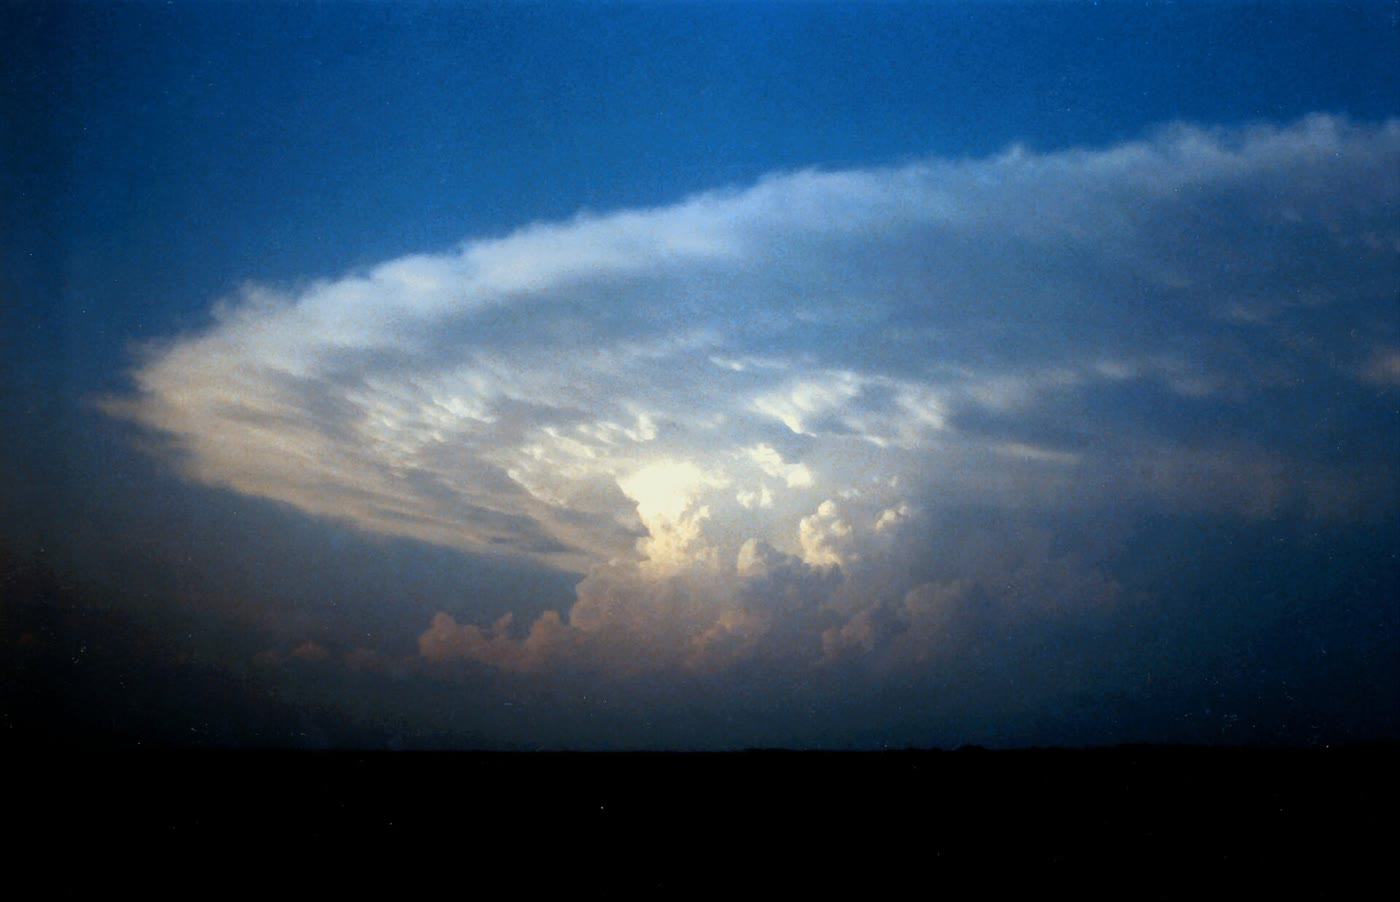
\includegraphics[width=0.6\linewidth]{images/book4/b2-21-supercell-anvil.jpg}
\par\smallskip{\small नेब्रास्का के ऊपर एक तड़ित-झंझा, 20 अप्रैल 1985: उसकी ऊर्ध्व धारा
एक निहाई में फैलती है जहाँ वह अपने \omterm{def:b2:atmospheric-thermodynamics:parcel-levels}{साम्य तल} तक पहुँचती है, क्षोभसीमा के पास। (Stephen Corfidi,
NOAA/NWS, सार्वजनिक डोमेन, विकिमीडिया कॉमन्स के माध्यम से।)}
\end{omfigure}
% ledger: nws4:lfc-el

\section{मेघ सूक्ष्मभौतिकी}\label{sec:b2:atmospheric-thermodynamics:microphysics}

अपने LCL पर वायु-पिंड जल की एक समतल सतह के ऊपर संतृप्त होता है। बूँद समतल नहीं होती: भौतिकी की
पुस्तकें दिखाती हैं कि नई प्रावस्था साम्य पर प्रकट नहीं होती, बल्कि केवल नाभिकन के द्वारा, और
रसायन विज्ञान की पुस्तकें कि वक्र सतह के ऊपर \omterm{def:b2:atmospheric-thermodynamics:moist-air}{वाष्प दाब} समतल सतह के ऊपर वाले से अधिक होता है
(केल्विन समीकरण)। नीचे के \cref{prop:b2:atmospheric-thermodynamics:kohler} के स्थिरांक $A$ के साथ,
\qty{2}{nm} व्यास की शुद्ध जल की बूँद केवल संतृप्ति-अनुपात
$\exp(2.1/2) = 2.9$ पर साम्य में होती है, यानी \qty{190}{\percent} की \omterm{def:b2:atmospheric-thermodynamics:microphysics}{अतिसंतृप्ति}, जो उन प्रतिशत के अंशों से कहीं ऊपर है
जिन पर कण सक्रियित होते हैं: बूँदें कणों पर बनती हैं।

\begin{definition}[अतिसंतृप्ति; मेघ संघनन केंद्रक]\label{def:b2:atmospheric-thermodynamics:microphysics}
वायु की \emph{अतिसंतृप्ति}\index{अतिसंतृप्ति} $s = e/e_s - 1$ है, यानी शुद्ध जल की समतल सतह के ऊपर के
संतृप्त \omterm{def:b2:atmospheric-thermodynamics:moist-air}{वाष्प दाब} पर उसके \omterm{def:b2:atmospheric-thermodynamics:moist-air}{वाष्प दाब} का आधिक्य, जो सामान्यतः
प्रतिशत में दिया जाता है। एक \emph{मेघ संघनन केंद्रक}\index{मेघ संघनन केंद्रक} (CCN)
वह एरोसॉल कण है जिस पर मेघों की छोटी अतिसंतृप्तियों पर मेघ-बूँद बनती है।
यही स्कूल की पुस्तकों का \emph{संघनन केंद्रक}\index{संघनन केंद्रक} है।
\end{definition}
% ledger: nws4:ccn-bergeron, pk07:kohler, morrison20:processes

\begin{proposition}[कोहलर वक्र]\label{prop:b2:atmospheric-thermodynamics:kohler}
\index{कोहलर वक्र}
व्यास $D$ की एक विलयन-बूँद, जो व्यास $D_d$ और आर्द्रताग्राहिता
$\kappa$ वाले एक शुष्क कण पर बढ़ी है, इस संतृप्ति-अनुपात के साथ साम्य में होती है:
\[
  S(D) = \frac{D^3 - D_d^3}{D^3 - D_d^3(1 - \kappa)}\,\exp\Bigl(\frac{A}{D}\Bigr), \qquad
  A = \frac{4\sigma M_w}{R T\rho_w},
\]
जहाँ $\sigma$ पृष्ठ तनाव है और $\rho_w$ जल का घनत्व (स्वीकृत)। वक्र $S(D)$
\emph{\omterm{prop:b2:atmospheric-thermodynamics:kohler}{कोहलर वक्र}} है। $D \gg D_d$ के लिए,
\[
  s = S - 1 \approx \frac{A}{D} - \frac{\kappa D_d^3}{D^3},
\]
जो क्रांतिक व्यास और \omterm{def:b2:atmospheric-thermodynamics:microphysics}{अतिसंतृप्ति} पर अधिकतम है:
\[
  D_c = \sqrt{\frac{3\kappa D_d^3}{A}}, \qquad s_c = \sqrt{\frac{4A^3}{27\,\kappa D_d^3}} .
\]
\end{proposition}
% ledger: pk07:kohler

\begin{proof}[सन्निकटन की उपपत्ति]
चरघातांकी केल्विन गुणक है; भिन्न जल-सक्रियता है, राउल्ट के नियम का एक रूप
जिसमें $\kappa$ मापता है कि घुला पदार्थ कितना जल बाँधता है। $D \gg D_d$ और
$A \ll D$ के लिए, $\exp(A/D) \approx 1 + A/D$ और भिन्न प्रथम कोटि तक $1 - \kappa D_d^3/D^3$ है;
गुणनफल, प्रथम कोटि तक, $1 + A/D - \kappa D_d^3/D^3$ है। अवकलज
$-A/D^2 + 3\kappa D_d^3/D^4$ को शून्य रखने पर $D_c^2 = 3\kappa D_d^3/A$ मिलता है, और तब $s_c = A/D_c -
A/(3D_c) = 2A/(3D_c)$, जो सूत्र है।
\end{proof}

$\sigma = \qty{0.072}{J/m^2}$ के साथ, \qty{298.15}{K} पर, $A = \qty{2.1}{nm}$। अमोनियम सल्फ़ेट का
$\kappa = 0.61$ है; सोडियम क्लोराइड और भी अधिक आर्द्रताग्राही है ($\kappa = 1.28$), और वायुमंडलीय कण अधिकतर 0.1 और 0.9 के बीच हैं।
अमोनियम सल्फ़ेट के \qty{50}{nm} के शुष्क कण का $D_c = \qty{0.33}{\micro m}$ और $s_c =
\qty{0.42}{\percent}$ है; \qty{100}{nm} वाले का, \qty{0.93}{\micro m} और \qty{0.15}{\percent}। यह
सन्निकटन सटीक अधिकतम से \qty{1}{\percent} से कम भिन्न है।
% ledger: pk07:kohler, pk07:kappa

\begin{omfigure}
\centering
% figdata/bachelor-2/thermo.py part kohler
\begin{tikzpicture}
\begin{semilogxaxis}[width=0.72\linewidth, height=5.6cm, xmin=0.03, xmax=10, ymin=-0.4,
  ymax=1.1, xlabel={बूँद का व्यास $D$ (\unit{\micro m})}, ylabel={अतिसंतृप्ति $s$
  (\unit{\percent})}, tick label style={font=\scriptsize}, label style={font=\small},
  log ticks with fixed point, legend style={font=\scriptsize, draw=none, fill=none},
  legend pos=north east, legend cell align=left, unbounded coords=discard]
\addplot[ocBlue, thick, densely dotted] table[x=D_um, y=s30] {figdata/out/bachelor-2-thermo-kohler.dat};
\addlegendentry{$D_d = \qty{30}{nm}$}
\addplot[ocBlue, thick] table[x=D_um, y=s50] {figdata/out/bachelor-2-thermo-kohler.dat};
\addlegendentry{$D_d = \qty{50}{nm}$}
\addplot[ocBlue, thick, dashed] table[x=D_um, y=s100] {figdata/out/bachelor-2-thermo-kohler.dat};
\addlegendentry{$D_d = \qty{100}{nm}$}
\addplot[only marks, mark=*, mark size=1.5pt, black] coordinates {(0.1542,0.914) (0.3309,0.4244)
  (0.9345,0.1499)};
\draw[black!45] (axis cs:0.03,0) -- (axis cs:10,0);
\draw[ocRed, densely dashed] (axis cs:0.03,0.5) -- (axis cs:10,0.5);
\node[font=\scriptsize, ocRed, anchor=north west] at (axis cs:2.2,0.5) {$s = \qty{0.5}{\percent}$};
\end{semilogxaxis}
\end{tikzpicture}
\par\smallskip{\small अमोनियम सल्फ़ेट कणों ($\kappa = 0.61$) के तीन शुष्क व्यासों के \omterm{prop:b2:atmospheric-thermodynamics:kohler}{कोहलर वक्र},
\qty{298.15}{K} पर, उनके क्रांतिक बिंदुओं (बिंदु) के साथ। \qty{0.5}{\percent}
\omterm{def:b2:atmospheric-thermodynamics:microphysics}{अतिसंतृप्ति} वाली वायु में \qty{50}{nm} और \qty{100}{nm} के कण असीमित रूप से बढ़ते हैं;
\qty{30}{nm} का कण एक धुंध-बूँद बना रहता है।}
\end{omfigure}
% ledger: pk07:kohler, pk07:kappa

वक्र कणों को बाँट देता है। उसके शिखर के नीचे बूँद स्थायी साम्य में होती है: यदि वह बढ़ती है,
तो वायु उसके लिए पर्याप्त अतिसंतृप्त नहीं रहती और वह वापस सिकुड़ जाती है; ऐसी धुंध-बूँदें आर्द्रता के साथ फूलती
और सिकुड़ती हैं। एक बार वायु की \omterm{def:b2:atmospheric-thermodynamics:microphysics}{अतिसंतृप्ति} $s_c$ से अधिक हो जाए, तो बूँद
\emph{सक्रियित} होती है: शिखर के पार, बढ़ने के साथ उसे कम से कम \omterm{def:b2:atmospheric-thermodynamics:microphysics}{अतिसंतृप्ति} चाहिए, और वह
तब तक बढ़ती है जब तक वाष्प है। उठता वायु-पिंड ठंडा होता है, उसकी \omterm{def:b2:atmospheric-thermodynamics:microphysics}{अतिसंतृप्ति} चढ़ती है, और सबसे बड़े
और सबसे घुलनशील कण पहले सक्रियित होते हैं; उनसे बनी बूँदें फिर वाष्प ले लेती हैं और
\omterm{def:b2:atmospheric-thermodynamics:microphysics}{अतिसंतृप्ति} को सीमित कर देती हैं। दूरस्थ महासागरों के ऊपर \qty{0.4}{\percent} पर सक्रिय लगभग 110 CCN प्रति घन सेंटीमीटर
होते हैं, दूरस्थ महाद्वीपों के ऊपर लगभग दुगुने, और प्रदूषित वायु में लगभग
दस गुना अधिक। अधिक बूँदों में बँटा वही जल उन्हें छोटा बनाता है।
% ledger: andreae09:ccn, morrison20:processes

\begin{remark}[केवल संघनन वर्षा क्यों नहीं बनाता]\label{rem:b2:atmospheric-thermodynamics:growth}
बूँद अपनी ओर वाष्प के विसरण से बढ़ती है। त्रिज्या $r$ की बूँद के चारों ओर एक गोले से
फ़्लक्स $4\pi r D_v\,\Delta\rho_v$ है, जहाँ $D_v$ वाष्प की विसरणशीलता है और
$\Delta\rho_v$ दूर वाष्प-घनत्व का आधिक्य, इसलिए उसका द्रव्यमान $\tfrac43\pi r^3\rho_w$
$r$ के समानुपाती दर से बढ़ता है: $r\,\mathrm{d}r/\mathrm{d}t$ स्थिर है और $r^2$ समय में रैखिक रूप से
बढ़ता है। बड़ी बूँदें छोटी बूँदों से धीरे बढ़ती हैं, और केवल संघनन से बढ़ती समष्टि
संकरी होती है, चौड़ी नहीं। वर्षा-बूँदें तब बनती हैं जब भिन्न आकारों की बूँदें, भिन्न
चालों से गिरती हुई, टकराती और संलयित होती हैं।
\end{remark}
% ledger: morrison20:processes

\qty{0}{\celsius} तल के ऊपर मेघ अतिशीतित बूँदों से बना रहता है जब तक हिम-नाभिकीय
कण हिम-क्रिस्टल आरंभ नहीं करते। तब संतृप्ति वाले चित्र के दाएँ पैनल का
अंतर कार्य करता है: बूँदों के ऊपर संतृप्त वायु हिम के ऊपर
\qty{10}{\percent} अतिसंतृप्त है, \qty{-10}{\celsius} पर, उन अतिसंतृप्तियों के दसियों गुना जिन पर बूँदें सक्रियित हुई थीं।
क्रिस्टल बूँदों की क़ीमत पर निक्षेपण से बढ़ते हैं, जो वाष्पित होती हैं (बर्जरॉन
प्रक्रम, स्कूल की पुस्तकों का हिम-क्रिस्टल प्रक्रम), और वे बूँदों को एकत्र करते हैं जो उन पर
जम जाती हैं (राइमिंग)।
% ledger: nws4:ccn-bergeron, morrison20:processes, iapws4:sublimation

\begin{omfigure}
\centering
\begin{tikzpicture}[font=\scriptsize, box/.style={draw=black!60, rounded corners=2pt,
  align=center, minimum height=0.95cm, text width=2.1cm, fill=#1}, box/.default=white,
  >=Stealth]
\node[anchor=west, black!60] at (-1.15,0.8) {उष्ण प्रक्रम};
\node[box=black!6] (ccn) at (0,0) {एरोसॉल कण\\(CCN)};
\node[box=ocBlue!8] (haze) at (4.2,0) {धुंध-बूँद\\$s < s_c$};
\node[box=ocBlue!15] (act) at (8.4,0) {सक्रियित बूँद\\$s > s_c$};
\node[box=ocBlue!25] (rain) at (12.6,0) {वर्षा-बूँद};
\draw[->] (ccn) -- node[above] {आर्द्रता} (haze);
\draw[->] (haze) -- node[above] {आरोहण} (act);
\draw[->] (act) -- node[above, align=center] {संघट्ट,\\संलयन} (rain);
\node[anchor=west, black!60] at (-1.15,-3.4) {हिम प्रक्रम};
\node[box=black!6] (inp) at (0,-2.6) {हिम-नाभिकीय\\कण};
\node[box=omMeth!10] (ice) at (4.2,-2.6) {हिम-क्रिस्टल\\\qty{0}{\celsius} से नीचे};
\node[box=omMeth!20] (snow) at (8.4,-2.6) {हिम, ग्रॉपेल};
\node[box=ocBlue!25] (rain2) at (12.6,-2.6) {वर्षा};
\draw[->] (inp) -- (ice);
\draw[->] (ice) -- node[above, align=center] {निक्षेपण,\\राइमिंग} (snow);
\draw[->] (snow) -- node[above] {पिघलना} (rain2);
\draw[->, omMeth!60!black, dashed] (act.south) -- node[pos=0.45, right=4pt, align=left,
  omMeth!60!black] {\hspace{2.2em}वाष्पित होती बूँदों\\से वाष्प} (ice.north);
\end{tikzpicture}
\par\smallskip{\small वाष्प से वर्षण तक के दो मार्ग: बूँदों का सक्रियण और वृद्धि,
फिर संघट्ट और संलयन (ऊपर); हिम-क्रिस्टल जो अतिशीतित बूँदों की क़ीमत पर बढ़ते हैं,
राइमिंग करते हैं, और गर्म वायु में गिरते हुए पिघलते हैं (नीचे)।}
\end{omfigure}
% ledger: morrison20:processes, nws4:ccn-bergeron

\begin{inthefield}[एक सुबह का प्रक्षेपण]
\begin{minipage}[t]{0.54\linewidth}\vspace{0pt}
हर ऊपरी-वायु केंद्र पर तकनीशियन 00 और 12 UTC से पहले के घंटे में गुब्बारा और रेडियोसॉन्ड
तैयार करता है, वे समय जब विश्व के आठ सौ से अधिक केंद्र एक साथ प्रेक्षण
करते हैं। 60 से \qty{80}{g} का उपकरण गुब्बारे के नीचे लटकता है और दाब,
तापमान, आर्द्रता और अपनी उपग्रह-स्थिति हर सेकंड भेजता है। गुब्बारा लगभग
\qty{300}{m} प्रति मिनट उठता है, दो घंटे या अधिक तक, फटने से पहले \qty{35}{km} से आगे तक, और
\qty{300}{km} से अधिक बह सकता है। पूर्वानुमानकर्ता परिच्छेदिका को स्क्यू-T आरेख पर खींचते हैं, और जिन
दिनों तीव्र मौसम की आशंका होती है उन दिनों कुछ केंद्र अतिरिक्त गुब्बारे छोड़ते हैं।
\end{minipage}\hfill
\begin{minipage}[t]{0.42\linewidth}\vspace{0pt}
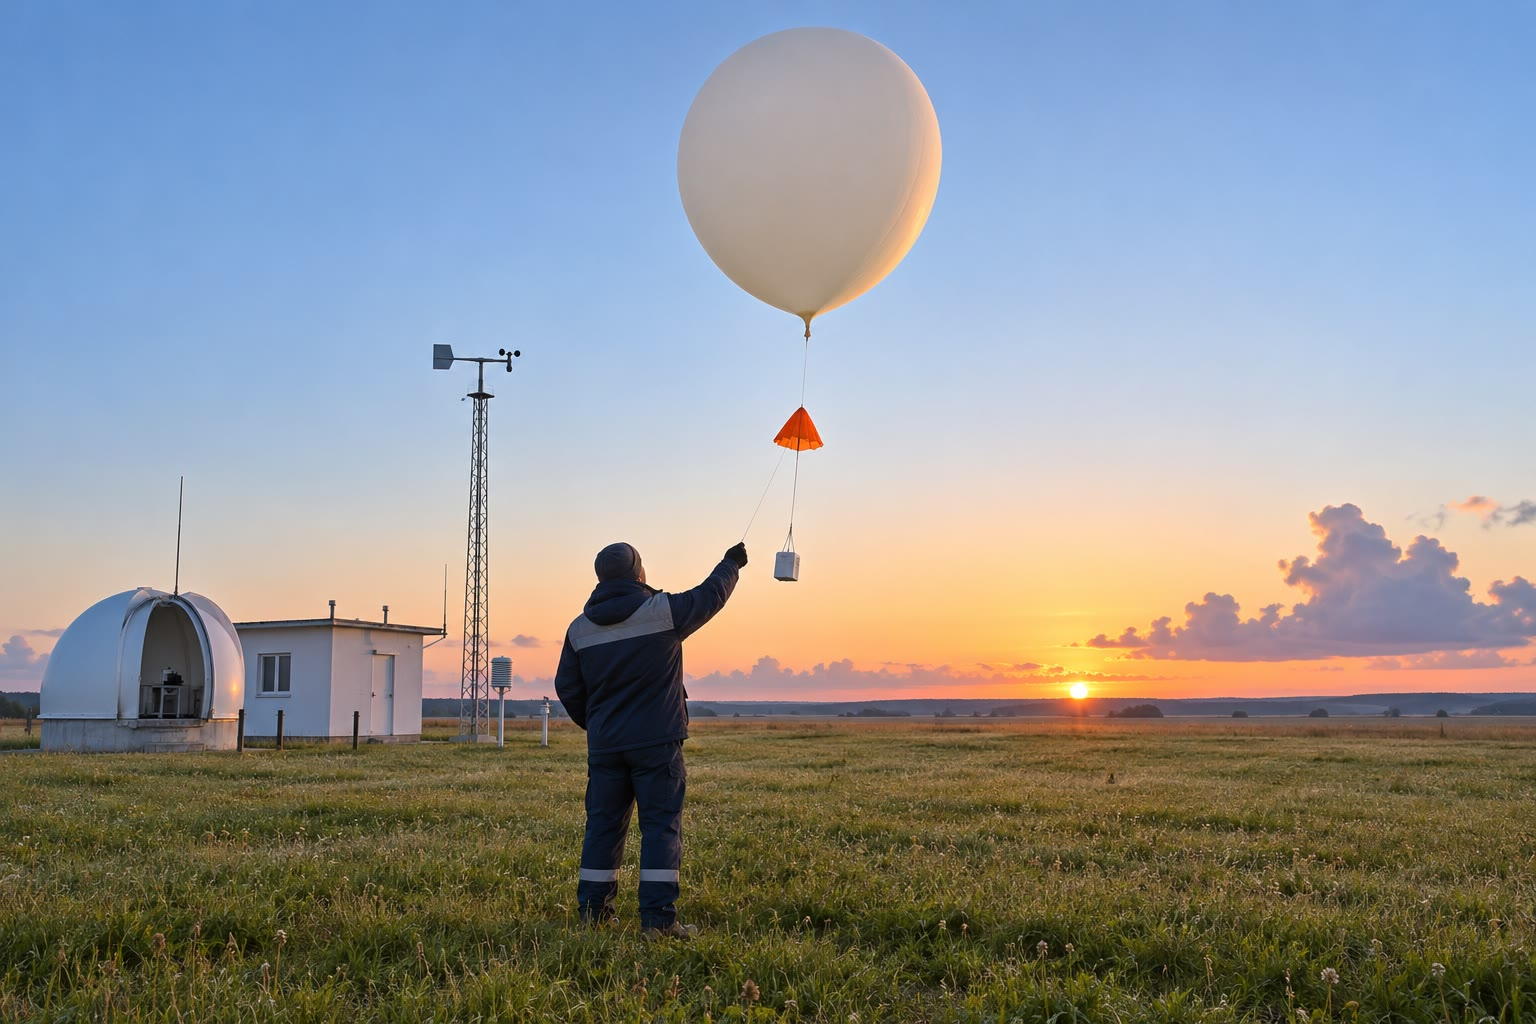
\includegraphics[width=\linewidth]{images/book4/ai/b2-radiosonde-launch.jpg}

{\scriptsize मौसम केंद्र से भोर में छोड़ा गया एक रेडियोसॉन्ड (AI-जनित
चित्रण)।}
\end{minipage}
% ledger: nws:radiosonde, nws4:upperair
\end{inthefield}

\section*{अभ्यास}\label{sec:b2:atmospheric-thermodynamics:exercises}

अभ्यासों के आँकड़े, अन्यथा न कहा जाए तो: $e_s(T) = \qty{6.117}{hPa} \times
\exp[\qty{5419}{K} \times (1/\qty{273.16}{K} - 1/T)]$; $\varepsilon = 0.622$, $R_d =
\qty{287.0}{J.kg^{-1}.K^{-1}}$, $R_v = \qty{461.5}{J.kg^{-1}.K^{-1}}$, $c_p =
\qty{1004.5}{J.kg^{-1}.K^{-1}}$, $L = \qty{2.501e6}{J/kg}$, $g = \qty{9.81}{m.s^{-2}}$,
$\Gamma_d = \qty{9.8}{K/km}$।
% ledger: nist4:water-sat, iapws4:sublimation, const:R, earth:Mmol, nist4:water-mw, nasa:grc-gamma

\begin{exercise}[$\star$]\label{exo:b2:atmospheric-thermodynamics:1}
\qty{850}{hPa} पर तापमान \qty{10.0}{\celsius} है और ओसांक \qty{5.0}{\celsius}।
(क)~\omterm{def:b2:atmospheric-thermodynamics:moist-air}{वाष्प दाब} और संतृप्त \omterm{def:b2:atmospheric-thermodynamics:moist-air}{वाष्प दाब} ज्ञात कीजिए। (ख)~सापेक्ष आर्द्रता ज्ञात कीजिए।
(ग)~\omterm{def:b2:atmospheric-thermodynamics:moist-air}{मिश्रण-अनुपात} और \omterm{def:b2:atmospheric-thermodynamics:moist-air}{विशिष्ट आर्द्रता} ग्राम प्रति किलोग्राम में ज्ञात कीजिए।
\end{exercise}

\begin{exercise}[$\star$]\label{exo:b2:atmospheric-thermodynamics:2}
(क)~$e_s$ प्रति केल्विन कितने प्रतिशत बढ़ता है, \qty{0}{\celsius}, \qty{20}{\celsius} और
\qty{30}{\celsius} पर? (ख)~$e_s$ की गणना \qty{20}{\celsius} और \qty{25}{\celsius} पर कीजिए, और उनका
अनुपात; $1.063^5$ से तुलना कीजिए। (ग)~\qty{20}{\celsius} पर मापा गया मान
\qty{23.39}{hPa} है। सूत्र कितनी त्रुटि करता है, और किस दिशा में? क्यों?
\end{exercise}
% ledger: nist4:water-sat

\begin{exercise}[$\star$]\label{exo:b2:atmospheric-thermodynamics:3}
दोपहर में सतही वायु \qty{30}{\celsius} पर है, \qty{14}{\celsius} के ओसांक के साथ। (क)~भूमि से
कितनी ऊँचाई पर कपासी मेघों के आधार बनते हैं? (ख)~शुष्क रुद्धोष्म वक्र से वहाँ वायु-पिंड का तापमान
क्या है? (ग)~$\Gamma_{\text{ओस}} =
\qty{1.8}{K/km}$ के साथ वहाँ उसका ओसांक क्या है? टिप्पणी कीजिए। (घ)~बाद में वायु \qty{33}{\celsius} तक गर्म होती है, ओसांक
अपरिवर्तित। अब मेघ-आधार कहाँ हैं?
\end{exercise}

\begin{exercise}[$\star$]\label{exo:b2:atmospheric-thermodynamics:4}
नॉर्मन साउंडिंग का स्क्यू-T आरेख पढ़िए। (क)~किस दाब तक भूमि के पास की वायु
संतृप्त, या लगभग संतृप्त, है? (ख)~व्युत्क्रमण कहाँ है, और वह कैसे दिखता है? (ग)~सतही वायु-पिंड के
LCL, LFC और EL पढ़िए। (घ)~व्युत्क्रमण के ठीक ऊपर ओसांक और तापमान की
तुलना कैसी है, और यह इस वायु के बारे में क्या कहता है?
\end{exercise}
% ledger: data:b4-sounding

\begin{exercise}[$\star\star$]\label{exo:b2:atmospheric-thermodynamics:5}
\qty{1000}{hPa} पर उष्णकटिबंधीय वायु का $T = \qty{30.0}{\celsius}$ और $r = \qty{20}{g/kg}$ है। (क)~उसका
\omterm{def:b2:atmospheric-thermodynamics:virtual}{आभासी तापमान} सटीक रूप से और सन्निकटन $T(1 + 0.61\,r)$ से ज्ञात कीजिए। (ख)~उसी तापमान और दाब पर इस वायु
के और शुष्क वायु के घनत्व ज्ञात कीजिए। (ग)~उतनी ही हल्की होने के लिए शुष्क वायु को कितना
गर्म करना पड़ेगा? (घ)~गर्म समुद्रों के ऊपर संवहन के लिए इसका क्या महत्त्व है?
\end{exercise}

\begin{exercise}[$\star\star$]\label{exo:b2:atmospheric-thermodynamics:6}
\qty{1000}{hPa} पर \cref{prop:b2:atmospheric-thermodynamics:gamma-s} का उपयोग कीजिए,
\cref{prop:b2:atmospheric-thermodynamics:humidity} से $r_s$ लेकर। (क)~$r_s$ और $\Gamma_s$ की गणना
\qty{0}{\celsius}, \qty{20}{\celsius} और \qty{30}{\celsius} पर कीजिए। (ख)~\qty{20}{\celsius} पर एक संतृप्त वायु-पिंड
\qty{1}{km} उठने के बाद शुष्क वायु-पिंड से कितना गर्म है, यदि उसकी तापह्रास दर
वही रहे? (ग)~ऊपर जाने पर अंतर क्यों घटता है?
\end{exercise}

\begin{exercise}[$\star\star$]\label{exo:b2:atmospheric-thermodynamics:7}
नॉर्मन के सतही वायु-पिंड ($p = \qty{971.1}{hPa}$, $T = \qty{19.0}{\celsius}$, $T_d =
\qty{18.5}{\celsius}$) का LCL \qty{18.35}{\celsius} पर है। (क)~उसके \omterm{def:b2:atmospheric-thermodynamics:moist-air}{मिश्रण-अनुपात}, उसके
विभव तापमान और उसके \omterm{def:b2:atmospheric-thermodynamics:theta-e}{समतुल्य विभव तापमान} की गणना कीजिए। (ख)~उठाए जाने पर वह
\qty{-8.9}{\celsius} पर है, \qty{500}{hPa} पर, संतृप्त। वहाँ उसके $\theta$ और $\theta_e$ की गणना कीजिए।
(ग)~दोनों में से कौन संरक्षित है?
\end{exercise}
% ledger: data:b4-sounding

\begin{exercise}[$\star\star$]\label{exo:b2:atmospheric-thermodynamics:8}
एक वायु-पिंड अपने परिवेश से \qty{4}{K} गर्म है, \qty{700}{hPa}, उसके LFC, और
\qty{300}{hPa}, उसके EL, के बीच; आभासी-तापमान सुधार की उपेक्षा कीजिए। (क)~उसके CAPE की गणना कीजिए। (ख)~$w_{\max}$
की गणना कीजिए। (ग)~CAPE किस श्रेणी में आता है? (घ)~स्क्यू-T आरेख पर धनात्मक क्षेत्रफल का
आकार क्या है, और उसका क्षेत्रफल वही क्यों है जो परिकलित किया गया?
\end{exercise}
% ledger: hgx:cape

\begin{exercise}[$\star\star$]\label{exo:b2:atmospheric-thermodynamics:9}
$A = \qty{2.1}{nm}$ और अमोनियम सल्फ़ेट, $\kappa = 0.61$, लीजिए। (क)~\qty{80}{nm} के एक शुष्क कण का
क्रांतिक व्यास और \omterm{def:b2:atmospheric-thermodynamics:microphysics}{अतिसंतृप्ति} ज्ञात कीजिए। (ख)~\qty{0.3}{\percent} \omterm{def:b2:atmospheric-thermodynamics:microphysics}{अतिसंतृप्ति} वाली वायु में सक्रियित होने वाला
सबसे छोटा शुष्क कण क्या है? \qty{0.1}{\percent} पर? (ग)~एक ऊर्ध्व धारा
\omterm{def:b2:atmospheric-thermodynamics:microphysics}{अतिसंतृप्ति} को \qty{0.1}{\percent} से \qty{0.3}{\percent} तक बढ़ाती है: बूँदों की संख्या का,
और उतने ही द्रव जल के लिए उनके आकार का, क्या होता है?
\end{exercise}
% ledger: pk07:kappa, pk07:kohler

\begin{exercise}[$\star\star\star$]\label{exo:b2:atmospheric-thermodynamics:10}
नॉर्मन के सतही वायु-पिंड का \omterm{def:b2:atmospheric-thermodynamics:virtual}{आभासी तापमान} के साथ CIN लगभग \qty{-130}{J/kg} था।
(क)~अपने ही संवेग से अपने LFC तक पहुँचने के लिए उसे किस ऊर्ध्वाधर चाल से भूमि छोड़नी होती?
(ख)~व्युत्क्रमण का शीर्ष \qty{889.1}{hPa} और \qty{20.5}{\celsius} पर है। \qty{971.1}{hPa} पर सतही वायु
को किस तापमान तक गर्म होना होगा ताकि शुष्क-रुद्धोष्म रूप से उठाया गया वायु-पिंड
व्युत्क्रमण के शीर्ष से ठंडा न हो? (ग)~यदि उसका ओसांक
\qty{18.5}{\celsius} पर रहता, तो उसका मेघ-आधार कहाँ होता? (घ)~दो ऐसे तरीके बताइए जिनसे वायुमंडल
सूर्य के बिना ऐसे ढक्कन को हटाता है।
\end{exercise}
% ledger: data:b4-sounding, nws4:cin

\begin{exercise}[$\star\star\star$]\label{exo:b2:atmospheric-thermodynamics:11}
(क)~\cref{prop:b2:atmospheric-thermodynamics:gamma-s} से दिखाइए कि $\Gamma_s \to \Gamma_d$ जब $r_s \to 0$।
(ख)~दिखाइए कि जब $Lr_s/(R_dT) \gg 1$, तब $\Gamma_s \to gR_vT/(LR_d)$, और
\qty{303}{K} पर उसका मान निकालिए। (ग)~\cref{prop:b2:atmospheric-thermodynamics:lcl} के
$\Gamma_{\text{ओस}}$ से तुलना कीजिए जब $T_d = T$, और समझाइए कि दोनों सीमाएँ
क्यों मेल खाती हैं। (घ)~क्या (ख) की सीमा वायुमंडल में पहुँची जाती है? मान $\Gamma_s =
\qty{3.4}{K/km}$ का उपयोग कीजिए, \qty{30}{\celsius} और \qty{1000}{hPa} पर।
\end{exercise}

\begin{exercise}[$\star\star\star$]\label{exo:b2:atmospheric-thermodynamics:12}
अतिशीतित जल के ऊपर और हिम के ऊपर संतृप्त \omterm{def:b2:atmospheric-thermodynamics:moist-air}{वाष्प दाब} 2.868 और
\qty{2.599}{hPa} हैं \qty{-10}{\celsius} पर, 1.257 और \qty{1.032}{hPa} \qty{-20}{\celsius} पर।
(क)~दोनों तापमानों पर जल के ऊपर संतृप्त वायु की हिम के ऊपर \omterm{def:b2:atmospheric-thermodynamics:microphysics}{अतिसंतृप्ति} ज्ञात कीजिए। (ख)~उन
अतिसंतृप्तियों से तुलना कीजिए जिन पर बूँदें सक्रियित होती हैं। (ग)~समझाइए कि कुछ हिम-क्रिस्टल पाने वाला
अतिशीतित बूँदों का मेघ हिम में क्यों बदल जाता है। (घ)~\qty{0}{\celsius} के पास प्रभाव
क्यों कमज़ोर है?
\end{exercise}
% ledger: iapws4:sublimation, su26:svp, nws4:ccn-bergeron

\begin{problem}[{सप्ताहांत समस्या --- सुबह की साउंडिंग पढ़ना}]\label{pb:b2:atmospheric-thermodynamics:1}
तालिका नॉर्मन, ओक्लाहोमा की 16 अप्रैल 2026 की 12 UTC साउंडिंग देती है, यहाँ प्रयुक्त
तलों पर: दाब, समुद्र-तल से ऊँचाई, तापमान, ओसांक, और
\cref{met:b2:atmospheric-thermodynamics:lift} की तरह उठाए गए सतही वायु-पिंड का तापमान, जो
\cref{prop:b2:atmospheric-thermodynamics:gamma-s} को छोटे चरणों में समाकलित करके परिकलित है। साउंडिंग
क्षोभसीमा को \qty{235.3}{hPa} और \qty{10954}{m} पर बताती है। अभ्यासों के आँकड़ों का और
तापमानों (\omterm{def:b2:atmospheric-thermodynamics:virtual}{आभासी तापमानों} का नहीं) का उपयोग कीजिए, जब तक अन्यथा न कहा जाए।

\begin{center}
\small
\begin{tabular}{rrrrr}
\hline
$p$ (\unit{hPa}) & $z$ (\unit{m}) & $T$ (\unit{\celsius}) & $T_d$ (\unit{\celsius}) &
$T_{\text{पिंड}}$ (\unit{\celsius}) \\
\hline
971.1 & 345 & 19.0 & 18.5 & 19.0 \\
925.0 & 763 & 17.3 & 17.3 & 16.9 \\
907.7 & 924 & 16.4 & 16.4 & 16.2 \\
889.1 & 1102 & 20.5 & 9.5 & 15.4 \\
850.0 & 1489 & 18.6 & $-1.8$ & 13.7 \\
700.0 & 3110 & 4.5 & $-12.2$ & 6.1 \\
500.0 & 5725 & $-18.4$ & $-36.6$ & $-8.9$ \\
400.0 & 7357 & $-30.4$ & $-55.6$ & $-20.4$ \\
300.0 & 9349 & $-42.7$ & $-66.3$ & $-37.1$ \\
250.0 & 10560 & $-49.8$ & $-69.8$ & $-48.3$ \\
200.0 & 12006 & $-52.3$ & $-78.3$ & $-61.8$ \\
\hline
\end{tabular}
\end{center}

\medskip\noindent\textbf{भाग I --- भूमि के पास की वायु।}
\begin{enumerate}
  \item सतही वायु का \omterm{def:b2:atmospheric-thermodynamics:moist-air}{वाष्प दाब} एक दशमलव तक ज्ञात कीजिए।
  \item उसका \omterm{def:b2:atmospheric-thermodynamics:moist-air}{मिश्रण-अनुपात} एक दशमलव तक ज्ञात कीजिए।
  \item उसकी \omterm{def:b2:atmospheric-thermodynamics:moist-air}{विशिष्ट आर्द्रता} ज्ञात कीजिए।
  \item उसकी सापेक्ष आर्द्रता ज्ञात कीजिए।
  \item उसका \omterm{def:b2:atmospheric-thermodynamics:virtual}{आभासी तापमान} उसके तापमान से कितना अधिक है?
  \item \qty{125}{m} के नियम से भूमि के ऊपर उसके LCL की ऊँचाई ज्ञात कीजिए, और वहाँ का
        दाब (परत के लिए \qty{294.7}{K} का माध्य \omterm{def:b2:atmospheric-thermodynamics:virtual}{आभासी तापमान} लीजिए)।
  \item उसका विभव तापमान ज्ञात कीजिए।
\end{enumerate}

\medskip\noindent\textbf{भाग II --- ढक्कन और ऊपर की परतें।}
\begin{enumerate}[resume]
  \item \qty{925}{hPa} पर वायु-पिंड अपने परिवेश से गर्म है या ठंडा, और कितना?
  \item 907.7 और \qty{889.1}{hPa} के बीच तापह्रास दर ज्ञात कीजिए। यह किस प्रकार की परत है?
  \item \qty{889.1}{hPa} पर वायु-पिंड अपने परिवेश से कितना ठंडा है?
  \item \qty{850}{hPa} पर सापेक्ष आर्द्रता ज्ञात कीजिए। ऐसी वायु कहाँ से आई हो सकती है?
  \item 850 और \qty{500}{hPa} के बीच माध्य तापह्रास दर ज्ञात कीजिए और परत का वर्गीकरण कीजिए।
  \item उत्थापित सूचकांक और उसकी श्रेणी ज्ञात कीजिए।
\end{enumerate}

\medskip\noindent\textbf{भाग III --- ऊर्जा।}
\begin{enumerate}[resume]
  \item तालिका के हर तल पर आधिक्य $\Delta T = T_{\text{पिंड}} - T$ की गणना कीजिए।
  \item $\Delta T$ का $\ln p$ में रैखिक अंतर्वेशन करके LFC को निकटतम हेक्टोपास्कल तक ज्ञात कीजिए,
        और उसी तरह $z$ का अंतर्वेशन करके उसकी ऊँचाई।
  \item उसी तरह EL और उसकी ऊँचाई ज्ञात कीजिए। क्षोभसीमा से तुलना कीजिए।
  \item $\ln p$ में समलंब नियम से, LFC से EL तक, तालिका के
        तलों से होते हुए, CAPE की गणना कीजिए।
  \item वह किस श्रेणी में आता है?
  \item उसी तरह भूमि से LFC तक CIN की गणना कीजिए।
  \item \qty{1}{hPa} के ग्रिड पर एक गणना तापमानों के साथ \qty{2100}{J/kg} और \omterm{def:b2:atmospheric-thermodynamics:virtual}{आभासी तापमानों} के साथ
        \qty{2230}{J/kg} का CAPE देती है। तीनों मान भिन्न
        क्यों हैं?
\end{enumerate}

\medskip\noindent\textbf{भाग IV --- वह तूफ़ान जिसे यह वायु पोषित कर सकती थी।}
\begin{enumerate}[resume]
  \item प्रश्न 17 के CAPE के साथ वायु-पिंड सिद्धांत कौन-सी ऊर्ध्वाधर चाल देता है?
  \item पूरे मार्ग में उसकी आधी चाल पर, वायु को LFC से EL तक उठने में कितना समय लगता?
  \item ऐसे दो प्रभाव बताइए जो वास्तविक ऊर्ध्व धारा को धीमा बनाते हैं।
  \item सारांश: इस सुबह की सतही वायु से पोषित तूफ़ान के लिए वायु-पिंड सिद्धांत कौन-सी ऊर्ध्व धारा चाल
        बताता है?
\end{enumerate}
\end{problem}
% ledger: data:b4-sounding, hgx:cape, nws4:lifted-index, nws4:cape
